\documentclass[12pt,english,dvipsnames,aspectratio=169,handout]{beamer}\usepackage[]{graphicx}\usepackage[]{xcolor}
% maxwidth is the original width if it is less than linewidth
% otherwise use linewidth (to make sure the graphics do not exceed the margin)
\makeatletter
\def\maxwidth{ %
  \ifdim\Gin@nat@width>\linewidth
    \linewidth
  \else
    \Gin@nat@width
  \fi
}
\makeatother

\definecolor{fgcolor}{rgb}{0.345, 0.345, 0.345}
\newcommand{\hlnum}[1]{\textcolor[rgb]{0.686,0.059,0.569}{#1}}%
\newcommand{\hlstr}[1]{\textcolor[rgb]{0.192,0.494,0.8}{#1}}%
\newcommand{\hlcom}[1]{\textcolor[rgb]{0.678,0.584,0.686}{\textit{#1}}}%
\newcommand{\hlopt}[1]{\textcolor[rgb]{0,0,0}{#1}}%
\newcommand{\hlstd}[1]{\textcolor[rgb]{0.345,0.345,0.345}{#1}}%
\newcommand{\hlkwa}[1]{\textcolor[rgb]{0.161,0.373,0.58}{\textbf{#1}}}%
\newcommand{\hlkwb}[1]{\textcolor[rgb]{0.69,0.353,0.396}{#1}}%
\newcommand{\hlkwc}[1]{\textcolor[rgb]{0.333,0.667,0.333}{#1}}%
\newcommand{\hlkwd}[1]{\textcolor[rgb]{0.737,0.353,0.396}{\textbf{#1}}}%
\let\hlipl\hlkwb

\usepackage{framed}
\makeatletter
\newenvironment{kframe}{%
 \def\at@end@of@kframe{}%
 \ifinner\ifhmode%
  \def\at@end@of@kframe{\end{minipage}}%
  \begin{minipage}{\columnwidth}%
 \fi\fi%
 \def\FrameCommand##1{\hskip\@totalleftmargin \hskip-\fboxsep
 \colorbox{shadecolor}{##1}\hskip-\fboxsep
     % There is no \\@totalrightmargin, so:
     \hskip-\linewidth \hskip-\@totalleftmargin \hskip\columnwidth}%
 \MakeFramed {\advance\hsize-\width
   \@totalleftmargin\z@ \linewidth\hsize
   \@setminipage}}%
 {\par\unskip\endMakeFramed%
 \at@end@of@kframe}
\makeatother

\definecolor{shadecolor}{rgb}{.97, .97, .97}
\definecolor{messagecolor}{rgb}{0, 0, 0}
\definecolor{warningcolor}{rgb}{1, 0, 1}
\definecolor{errorcolor}{rgb}{1, 0, 0}
\newenvironment{knitrout}{}{} % an empty environment to be redefined in TeX

\usepackage{alltt}
\usepackage{fontspec}
\setsansfont[Mapping=tex-text]{Fira Sans}
\setcounter{secnumdepth}{4}
\setcounter{tocdepth}{4}
\usepackage[normalem]{ulem}
\usepackage[T1]{fontenc}
\usepackage{dcolumn}
\usepackage{booktabs}
\usepackage{bm}
\usepackage{setspace}
\makeatletter
\usetheme{metropolis}
\setbeamertemplate{frame footer}{Bosancianu | Schaub | Hertie School}
\setbeamerfont{page number in head/foot}{size=\tiny}
\setbeamercolor{footline}{fg=gray}
\usepackage{xcolor}
\setbeamercovered{transparent}
\usepackage{tikz}
\usetikzlibrary{arrows, positioning,fit,shapes.misc}
\usepackage[labelformat=empty]{caption}
% For table captions in Beamer
\usepackage[sectionbib]{apacite}
\renewcommand{\bibliographytypesize}{\footnotesize}
\makeatletter
\let\st@rtbibsection\@bibnewpage
\let\st@rtbibchapter\@bibnewpage
\makeatother
\usepackage{amsmath, mathtools}
\usepackage{xunicode}
\usepackage{hyperref}
\graphicspath{{./figures/}} 
% Defines a checkmark
\def\checkmark{\tikz\fill[scale=0.4,color=orange](0,.35) -- (.25,0) -- (1,.7) -- (.25,.15) -- cycle;}
% Code for circles in Table cells
\newcounter{nodemarkers}
\newcommand\circletext[1]{%
    \tikz[overlay,remember picture] 
        \node (marker-\arabic{nodemarkers}-a) at (0,1.5ex) {};%
    #1%
    \tikz[overlay,remember picture]
        \node (marker-\arabic{nodemarkers}-b) at (0,0){};%
    \tikz[overlay,remember picture,inner sep=2pt]
        \node[draw,ellipse,fit=(marker-\arabic{nodemarkers}-a.center) (marker-\arabic{nodemarkers}-b.center)] {};%
    \stepcounter{nodemarkers}%
}
% wide itemize and enumerate
\newenvironment{wideitemize}{\itemize\addtolength{\itemsep}{.3em}}{\enditemize}
\newenvironment{wideenumerate}{\enumerate\addtolength{\itemsep}{.3em}}{\endenumerate}
% boxes
\def\boxitorange#1{%
  \smash{\color{orange}\fboxrule=1pt\relax\fboxsep=2pt\relax%
  \llap{\rlap{\fbox{\vphantom{0}\makebox[#1]{}}}~}}\ignorespaces
}
\def\boxitblue#1{%
  \smash{\color{blue}\fboxrule=1pt\relax\fboxsep=2pt\relax%
  \llap{\rlap{\fbox{\vphantom{0}\makebox[#1]{}}}~}}\ignorespaces
}
\newcommand{\indep}{\perp \!\!\!\! \perp}
\setbeamertemplate{itemize items}{\checkmark}
\usepackage{multirow}
\hypersetup{pdfauthor={Bosancianu and Schaub},
	pdftitle={Statistical Modeling and Causal Inference with R},
	pdfsubject={Week 10: Moderation and heterogeneous effects},
	pdfkeywords={Berlin, Hertie, 2020, week 8}}
\title{\textsc{Statistical Modeling and Causal Inference with R}}
\subtitle{Week 10: Moderation and heterogeneous effects}
\date{November 16, 2020}
\author{Manuel Bosancianu \hfill Max Schaub}
\institute{Hertie School of Governance}
\IfFileExists{upquote.sty}{\usepackage{upquote}}{}
\begin{document}
\maketitle

\begin{frame}
	\frametitle{Today's focus}
	\begin{itemize}
		\item Motivation
		\item Moderation vs.\ mediation
		\item Understanding treatment heterogeneity
		\item Estimating heterogeneous treatment effects
		\item Caveats
	\end{itemize}
\end{frame}


\section{Motivation}

\begin{frame}
  \frametitle{Motivation}
\footnotesize

\begin{enumerate} 
\item[1.] Philosophical
    \begin{itemize} \scriptsize
    \item What sets the social sciences apart from many hard sciences is that we are \textcolor{orange}{population sciences} is that we are dealing with individuals who differ in manifold ways from each other \cite{xie_population_2013}. 
    \item One individual cannot `stand in' for the next, like e.g.\ molecules in chemistry. This is the reason why we have to make our inferences at the group level: while groups can be counterfactuals for each other, individuals rarely can. 
    \item Still it is somewhat paradoxical that in causal inference we often only estimate the average effect for all individuals, notwithstanding the fact that the recognition of individual differences are at the heart of our science. We would therefore clearly expect a treatment to have different effects for different individuals.
    \item The explicit modeling of heterogeneity in treatment effects for \textcolor{orange}{subgroups} addresses this tension between the necessity of having to do inference at the group level, and the recognition of individual differences.
    \end{itemize}
\end{enumerate}

\end{frame}


\begin{frame}
  \frametitle{Motivation}
\footnotesize

\begin{enumerate}
\item[2.] Inference:
    \begin{itemize} \footnotesize
    \item We commonly invoke the constant effects assumption  $E[Y_{1i}|D=1] =  E[Y_{0i}|D=0] + \kappa$, e.g.\ when using simple additive regression models for estimating treatment effects
    \item Where this assumption does not hold, results can be biased \cite{angrist_estimating_1998, elwert_effect_2010}
    \item To obtain consistent results, we therefore have to include interaction terms/allow for heterogeneity.
    \end{itemize}
\end{enumerate}
\vspace{3cm}

\end{frame}



\begin{frame}
  \frametitle{Motivation}
\footnotesize

\begin{enumerate}
\item[3.] Policy relevance: 
    \begin{itemize} \footnotesize
    \item Analysis of heterogeneity can be very important for policy
    \item The same treatment may be \textcolor{orange}{effective} have (beneficial) effects for one subgroup, but be harmful for another, e.g.\ certain types of surgeries. 
    \item Resources can be much more \textcolor{orange}{efficiently} spent if it is clear who reacts to a treatment, and who does not. 
    \end{itemize}
\end{enumerate}
\vspace{3cm}

\end{frame}




\begin{frame}
  \frametitle{Moderation vs. mediation}
\footnotesize
Mediator: variable that lies \textcolor{orange}{on the causal path} from treatment D to outcome Y; explains (part of) the effect 


	 \begin{figure} 
    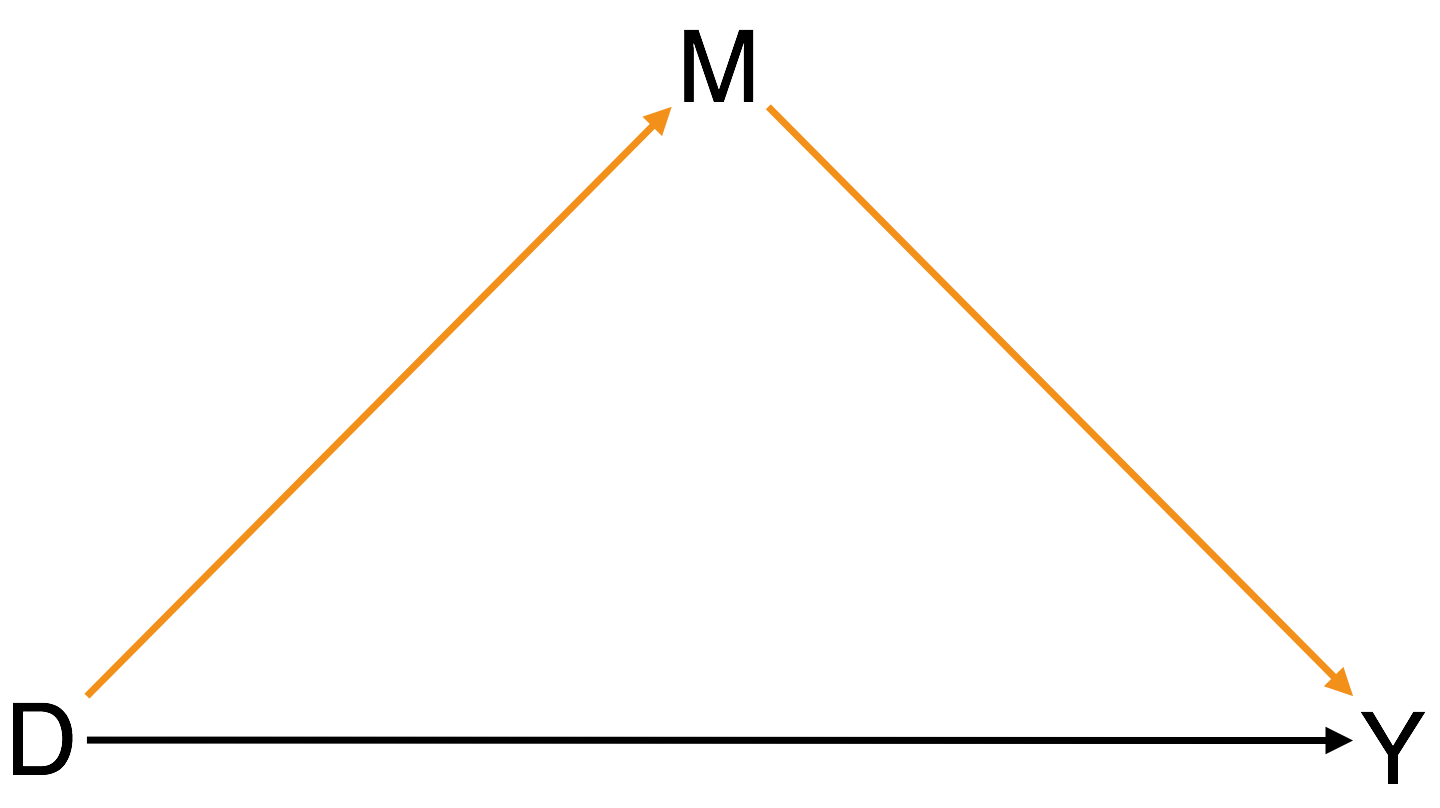
\includegraphics[height=.3\textheight,keepaspectratio=true]{../04-figures/10/01-w10_mediator}
    \end{figure}

Theme of next class!

\vspace{1cm}
\end{frame}


\begin{frame}
  \frametitle{Moderation vs. mediation}
\footnotesize
Moderator: variable that \textcolor{orange}{divides treated population in groups} among which the treatment D has differential effects

	 \begin{figure} 
    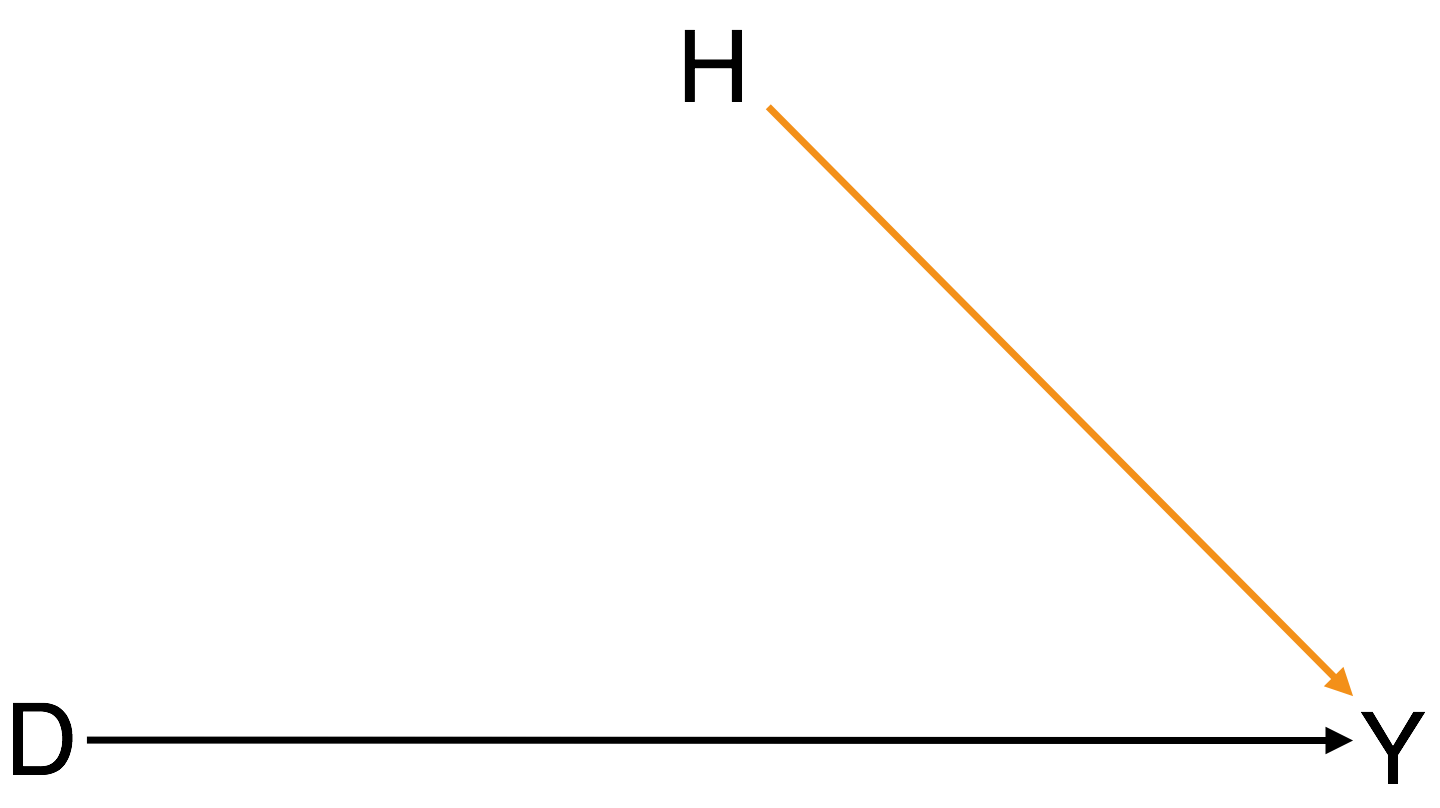
\includegraphics[height=.3\textheight,keepaspectratio=true]{../04-figures/10/02-w10_moderator}
    \end{figure}
    
DAGs not very well suited to depict moderation \cite[80]{hernan_causal_2021}; H could also be additional predictor that is independent of X; here meant to indicate effect modification/heterogeneity

\end{frame}


\begin{frame}
  \frametitle{Moderation vs. mediation}
\footnotesize
Moderators sometimes depicted as an arrow aimed at the arrow linking D and Y

	 \begin{figure} 
    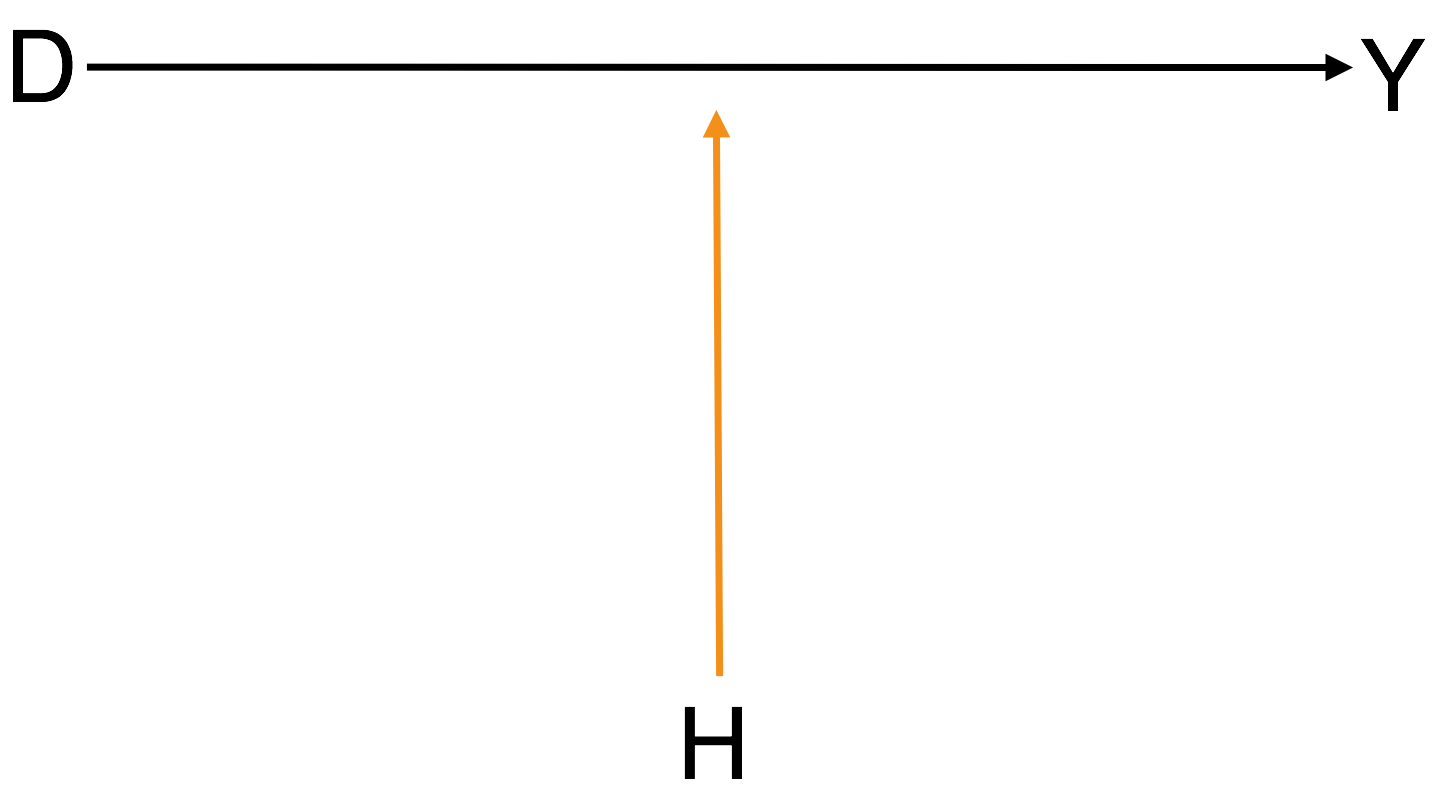
\includegraphics[height=.3\textheight,keepaspectratio=true]{../04-figures/10/03-w10_moderator_informal}
    \end{figure}
    
But note that this no longer is a DAG\ldots

\vspace{1cm}
\end{frame}


\begin{frame}
  \frametitle{Moderation vs. mediation}
\footnotesize

Different terms used for moderation, depending on scientific field:

\begin{itemize}\footnotesize
  \item Moderation
  \item Effect modification
  \item Interaction effects
  \item Conditional treatment effects
  \item Heterogeneous treatment effects
  \item Conditional average treatment effects (CATEs)
\end{itemize}

\vspace{1cm}
\end{frame}


\section{Understanding treatment heterogeneity}

\begin{frame}
  \frametitle{Understanding treatment heterogeneity}
\footnotesize
What is the issue? Consider the following two tables:

\tiny
\begin{table}\centering
\begin{tabular}{lcccc}
\toprule
\multicolumn{5}{c}{Constant treatment effects}   \\
\midrule
Individual & $Y_{0i}$ &  $Y_{1i}$  & $\delta_i$ & Age group   \\
\midrule
A          &   4    &    7     &   3      & Young        \\
B          &   3    &    6     &   3      & Young        \\
C          &   -1    &    2     &   3      & Young        \\
D          &   11    &    14     &   3      & Young        \\
E          &   2    &    5     &   3      & Old        \\
F          &   1    &    4     &   3      & Old        \\
G          &   4    &    7     &   3      & Old        \\
H          &   0    &    3     &   3      & Old        \\
\hline\hline
Av         &   3    &    6     &   3      &         \\
\bottomrule
\end{tabular}
\end{table}

\footnotesize
Homogeneous/constant treatment effect across subjects, as invoked by many proofs (e.g.\ use of OLS for estimating treatment effect)

\end{frame}


\begin{frame}
  \frametitle{Understanding treatment heterogeneity}
\footnotesize
What is the issue? Consider the following two tables:

\tiny
\begin{table}\centering
\begin{tabular}{lcccc}
\toprule
\multicolumn{5}{c}{Heterogeneous treatment effects}   \\
\midrule
Individual & $Y_{0i}$ &  $Y_{1i}$  & $\delta_i$ & Age group   \\
\midrule
A          &   0    &    7     &   7      & Young        \\
B          &   1    &    6     &   5      & Young        \\
C          &   0    &    2     &   2      & Young        \\
D          &   4    &    14    &   10     & Young        \\
E          &   4    &    5     &   1      & Old        \\
F          &   4    &    4     &   0      & Old        \\
G          &   7    &    7     &   0      & Old        \\
H          &   4    &    3     &   -1     & Old        \\
\hline\hline
Av         &   3    &    6     &   3      &         \\
\bottomrule
\end{tabular}
\end{table}

\footnotesize
Heterogeneous treatment effect, clearly patterned along a covariate. Effect only among young ($\delta_{Young}=6$), zero among older.

Potentially highly policy relevant, e.g.\ if effect of vaccine.

\end{frame}




\begin{frame}
  \frametitle{Understanding treatment heterogeneity}
\footnotesize
In reality, like the average treatment effect, heterogeneous treatment effects have to be estimated because we only ever observe one potential outcome.

\tiny
\begin{table}\centering
\begin{tabular}{lccc}
\toprule
\multicolumn{4}{c}{Heterogeneous treatment effects}   \\
\midrule
Individual & $Y_{0i}|D=0$ &  $Y_{1i}|D=1$   & Age group   \\
\midrule
A          &   0    &                & Young        \\
B          &   1    &                & Young        \\
C          &        &    2           & Young        \\
D          &        &    14          & Young        \\
E          &   4    &                & Old        \\
F          &        &    4           & Old        \\
G          &   7    &                & Old        \\
H          &        &    3           & Old        \\
\hline\hline
Av         &   3    &    5.75     &   2.75         \\
\bottomrule
\end{tabular}
\end{table}

\footnotesize
Here the estimated treatment effect is 5.75, with that for the young being 7.5, and that for the old -2.

\end{frame}




\begin{frame}
  \frametitle{Descriptive vs. causal conditional treatment effects}
\footnotesize

\begin{itemize}
  \item With randomization of $D_i$, the treatment is identified for all subgroups.
  \item However, unless the subgroups are the result of randomization, the factor along which heterogeneity is assessed does \emph{not} have a causal interpretation.
  \item This is because this factor could be capturing the effect of another variable
  \item You \emph{can} give a causal interpretation to your interaction effect if you are interacting two treatments that were both randomized. 
\end{itemize}
\vspace{1cm}

\end{frame}





\section{Estimation of heterogeneous treatment effects}

\begin{frame}
  \frametitle{Estimation of heterogeneous treatment effects}
\footnotesize
Heterogeneous treatment effects are usually estimated with regression models that include an interaction between the treatment and the moderator:

$Y_i = \beta_0 + \beta_1 D_i + \beta_2 H_i + \beta_3 H_i \times D_i + \epsilon_i$

Compare this to a conventional additive model in the form

$Y_i = \gamma_0 + \gamma_1 D_i + \gamma_2 H_i + \mu_i$

How are the coefficients in the different models to be interpreted?

\vspace{2cm}
\end{frame}


\begin{frame}
  \frametitle{Estimation of heterogeneous treatment effects}
\footnotesize

In the \textcolor{orange}{additive model}, as you know, $\gamma_1$ is the marginal effect of $D_i$ on $Y_i$:	

\begin{equation*}
\frac{\partial Y_i}{\partial D_i} = \gamma_1
\end{equation*}
and $\gamma_2$ is the marginal effect of $H_i$ on $Y_i$:

\begin{equation*}
\frac{\partial Y_i}{\partial H_i} = \gamma_2
\end{equation*}

i.e.\ the coefficients capture what happens to $Y_i$ if $D_i$ or $H_i$ increase by one unit, respectively.

\vspace{1cm}
\end{frame}



\begin{frame}
  \frametitle{Estimation of heterogeneous treatment effects}
\footnotesize

In contrast, in the \textcolor{orange}{interaction model}, the marginal effect of $D_i$ on $Y_i$ is:	

\begin{equation*}
\frac{\partial Y_i}{\partial D_i} = \beta_1 + \beta_3 H
\end{equation*}

meaning the effect of $D_i$ depends on $H_i$ -- which is what we are after, of course!

For a binary moderating variable (that takes values 0 and 1), the marginal effect of $D_i$ is $\beta_1 + \beta_3$ if the moderator is one.

The partial effect also implies that the marginal effect of $D_i$ on $Y_i$ is $\beta_1$ if $\beta_3 H$ is zero. In the case of a binary moderator, this coefficient is directly interpretable.

For a moderator that takes more than one value, plausible marginal effects should be calculated.

\end{frame}



\begin{frame}
  \frametitle{Estimation of heterogeneous treatment effects}
\footnotesize
To sum up, the parameters in an interaction model

$Y_i = \beta_0 + \beta_1 D_i + \beta_2 H_i + \beta_3 H_i \times D_i + \epsilon_i$

are interpreted as follows:

\scriptsize
$\beta_0$: Constant\\
$\beta_1$: Effect of $D_i$ on $Y_i$ if $H_i$ is zero.\\
$\beta_2$: Effect of $H_i$ on $Y_i$ if $D_i$ is zero.\\ 
$\beta_3$: Difference in treatment effects of $D_i$ depending on $H_i$.
\vspace{5mm}

In other words, in the binary case, $\beta_3$ is the difference-in-differences in means ($(E[Y_i|D=1,H=1] - E[Y_i|D=0,H=1]) - (E[Y_i|D=1,H=0] - E[Y_i|D=0,H=0])$, and the difference in regression slopes where the interacted variable is continuous.

\end{frame}



\begin{frame}
  \frametitle{Calculating and plotting CATEs}
\footnotesize

An example: Recall study on right-wing support following expansion of broadband coverage \cite{schaub_voter_2020}. 

Basic finding: broadband availability goes along with higher support for right-wing populists.

Does the finding hold for all demographics, e.g.\ age groups? In other words, is the effect of broadband access moderated by age?

We start with a binary moderator as in the following model

$Y_i = \beta_0 + \beta_1 {BB} + \beta_2 {Older}_i + \beta_3 {Older}_i \times {BB}_i + \epsilon_i$

where ${BB}$ indicates broadband availability, which can be high (1) or low (0), and ${Older}$ is an indicator that is 1 if an individual is 55 years or more, and 0 if else.

\end{frame}



\begin{frame}
  \frametitle{Calculating and plotting CATEs}
\footnotesize

\scriptsize
\centering
\begin{tabular}{l*{1}{c}}
\toprule
\multicolumn{2}{c}{Conditional effect of broadband access on right-wing support}\\
\midrule
BB ($\beta_1$)&    0.136\textsuperscript{***}\\
                &   (0.05)         \\
Older ($\beta_2$)        &    0.033         \\
                &   (0.08)         \\
Older $\times$ BB ($\beta_3$) &   -0.149\textsuperscript{*}  \\
                &   (0.08)         \\
Constant ($\beta_0$)       &    0.062         \\
                &   (0.04)         \\
\midrule
Observations    &     1,158         \\
\(R^{2}\)       &     0.03         \\
\bottomrule
\multicolumn{2}{l}{Standard errors in parentheses}\\
\multicolumn{2}{l}{\textsuperscript{*} \(p<0.10\), \textsuperscript{**} \(p<0.05\), \textsuperscript{***} \(p<0.01\)}\\
\end{tabular}

\end{frame}


\begin{frame}
  \frametitle{Calculating and plotting CATEs}
\footnotesize

What is the conditional average treatment effect for the non-old/the younger? 

That's the constitutive term for the treatment indicator $\beta_1$ -- which gives us the treatment indicator when the moderator is zero, i.e. $\beta_1 = 0.136$.

But is there an effect for the old at all (i.e.\ an effect different from zero)? The regression table cannot tell.

While we can calculate the treatment effect for the old from the table as 

\scriptsize
$(\beta_1 + \beta_3) = 0.136-0.149 = -0.013$\footnotesize, 

we cannot tell if this effect is statistically significant/different from zero. This is because we lack the standard error for this quantity of interest  i.e.\
\scriptsize
$\hat{\sigma}_{\frac{\partial Y_i}{\partial D_i}}= \sqrt{var(\hat{\beta_1}) + var(\hat{\beta_3}) + 2cov(\hat{\beta_1} \hat{\beta_3})}.$

\end{frame}


\begin{frame}
  \frametitle{Calculating and plotting CATEs}
\footnotesize
We can calculate this standard error with a Wald-Test of the hypothesis $H0: \beta_1 + \beta_3 = 0$, or by having R calculate the marginal effects:
\vspace{5mm}

\scriptsize
\centering
\begin{tabular}{l*{1}{c}}
\toprule
\multicolumn{2}{c}{Marginal effects of broadband access on right-wing support}\\
\midrule
if Older=0         &    0.136\textsuperscript{***}\\
                &   (0.05)         \\
if Older=1         &   -0.013         \\
                &   (0.07)         \\
\midrule
Observations    &     1,158         \\
\bottomrule
\multicolumn{2}{l}{Standard errors in parentheses}\\
\multicolumn{2}{l}{\textsuperscript{*} \(p<0.10\), \textsuperscript{**} \(p<0.05\), \textsuperscript{***} \(p<0.01\)}\\
\end{tabular}

\end{frame}



\begin{frame}
  \frametitle{Calculating and plotting CATEs}
\footnotesize

We can also plot the results:

	 \begin{figure} 
    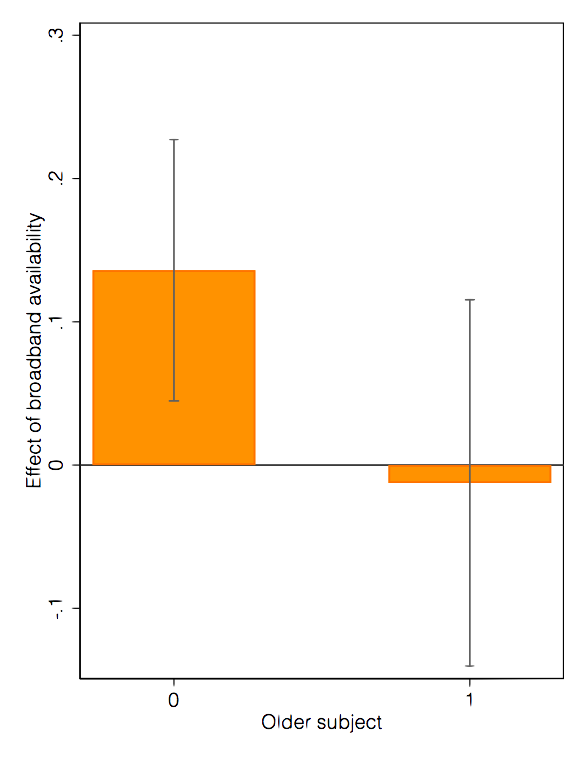
\includegraphics[height=.65\textheight,keepaspectratio=true]{../04-figures/10/04-w10_binary}
    \end{figure}

\vspace{1cm}
\end{frame}



\begin{frame}
  \frametitle{Calculating and plotting CATEs}
\footnotesize

Finally, we may ask if the differences in heterogeneous treatment effects are different, i.e.\ test $H0: \beta_1-(\beta_1 + \beta_3) = 0$ -- but that's $\beta_3$!

So we can just take this information from the regression table.

Here, despite the substantively big difference, this difference in treatment effect sizes is only marginally significant at p=0.06. 

This is because information becomes sparse the moment we start subdividing our sample.

\vspace{2cm}
\end{frame}


\begin{frame}
  \frametitle{Interaction term vs.\ split sample}
\footnotesize

Sometimes you see researchers \textcolor{orange}{splitting their sample}, i.e.\ calculate simple additive models for the different levels of the moderator variable. Is this legit?

The separate additive models and the interaction model are equivalent as long as only the treatment indicator $D_i$ and the moderator $H_i$ are included in the interaction model.

Once additional control variables are included, the interacted model and the split are \emph{no longer} equivalent.

This is because in the interacted model, all control variables are constrained to have the same effect for the full sample.

In the split model, control variables can have sample-specific effects.

The `split-model effect' can be emulated by including interaction terms for \emph{all} included control variables.

\end{frame}



\begin{frame}
  \frametitle{Interaction term vs.\ split sample}
\footnotesize
Consider again our example.

Without additional covariates, the split sample models recover the marginal effects calculated with the interaction model
\vspace{5mm}

\scriptsize
\centering
\begin{tabular}{l*{2}{c}}
\toprule
\multicolumn{3}{c}{Split-sample regression without additional covariates}\\
                & Older=0 &         Older=1 \\
\midrule
BB          &    0.136\textsuperscript{***}&   -0.013         \\
                &   (0.05)         &   (0.07)         \\
Constant        &    0.062         &    0.095         \\
                &   (0.04)         &   (0.06)         \\
\midrule
Observations    &      581         &      577         \\
\(R^{2}\)       &     0.01         &     0.00         \\
\bottomrule
\multicolumn{3}{l}{ Standard errors in parentheses}\\
\multicolumn{3}{l}{ \textsuperscript{*} \(p<0.10\), \textsuperscript{**} \(p<0.05\), \textsuperscript{***} \(p<0.01\)}\\
\end{tabular}

\end{frame}


\begin{frame}
  \frametitle{Interaction term vs.\ split sample}
\footnotesize
With \textcolor{orange}{additional covariates}, the interaction and the split sample model are \textcolor{orange}{no longer equivalent} because the treatment indicator interacts with the additional covariates in each subsample in different ways. 

\tiny
\centering
\begin{tabular}{l*{4}{c}}
\toprule
\multicolumn{5}{c}{Split-sample regression with additional covariates}\\
                & Older=0         & Older=1           &  Interaction  & All interacted \\
\midrule
BB              &    0.108\textsuperscript{**} &   -0.001         &    0.131\textsuperscript{***}&    0.108\textsuperscript{**} \\
                &   (0.05)         &   (0.07)         &   (0.05)         &   (0.05)         \\
Share w/ degree &    0.260         &   -0.141         &    0.049         &    0.260         \\
                &   (0.19)         &   (0.10)         &   (0.10)         &   (0.19)         \\
Older=1         &                  &                  &    0.031         &    0.170         \\
                &                  &                  &   (0.08)         &   (0.10)         \\
Older=1 $\times$ BB&               &                  &   -0.147\textsuperscript{*}  &   -0.108         \\
                &                  &                  &   (0.08)         &   (0.08)         \\
Older=1 $\times$ Share w/ degree&                  &                  &                  &   -0.401\textsuperscript{*}  \\
                &                  &                  &                  &   (0.21)         \\
Constant        &   -0.023         &    0.147\textsuperscript{**} &    0.046         &   -0.023         \\
                &   (0.07)         &   (0.07)         &   (0.05)         &   (0.07)         \\
\midrule
Observations    &      581         &      577         &     1,158         &     1,158         \\
\(R^{2}\)       &     0.01         &     0.00         &     0.03         &     0.03         \\
\bottomrule
\multicolumn{5}{l}{Standard errors in parentheses, \textsuperscript{*} \(p<0.10\), \textsuperscript{**} \(p<0.05\), \textsuperscript{***} \(p<0.01\)}\\
\end{tabular}

\end{frame}




\begin{frame}
  \frametitle{Interaction term vs.\ split sample}
\footnotesize

This coefficients of the split model + covariates can be recovered with the fully interacted model. This is rarely used in practice, however.
\vspace{5mm}

\tiny
\centering
\begin{tabular}{l*{4}{c}}
\toprule
\multicolumn{5}{c}{Marginal effects after split-sample regression with additional covariates}\\
                & Older=0         & Older=1           &  Interaction  & All interacted \\
\midrule
BB              &    0.108\textsuperscript{**} &   -0.001         &                  &                  \\
                &   (0.05)         &   (0.07)         &                  &                  \\
BB if Older=0   &                  &                  &    0.131\textsuperscript{***}&    0.108\textsuperscript{**} \\
                &                  &                  &   (0.05)         &   (0.05)         \\
BB if Older=1   &                  &                  &   -0.017         &   -0.001         \\
                &                  &                  &   (0.07)         &   (0.07)         \\
\midrule
Observations    &      581         &      577         &     1,158         &     1,158         \\
\bottomrule
\multicolumn{5}{l}{ Standard errors in parentheses}\\
\multicolumn{5}{l}{\textsuperscript{*} \(p<0.10\), \textsuperscript{**} \(p<0.05\), \textsuperscript{***} \(p<0.01\)}\\
\end{tabular}

\vspace{1cm}
\end{frame}


\begin{frame}
  \frametitle{Calculating and plotting CATEs}
\footnotesize

In \textcolor{orange}{treatment-by-treatment interactions} (i.e.\ where we manipulated two treatments simultaneously), while all the above applies, we are usually interested in the marginal effect of all the interaction terms. Consider the model $Y_i = \beta_0 + \beta_1 D_i^1 + \beta_2 D_i^2+ \beta_3 D_i^1 \times D_i^2 + \epsilon_i$

with the two treatments $D_i^1$ and $D_i^2$. 

These define four outcomes:

\scriptsize
\centering
\begin{tabular}{ll}
$(E[Y_i|D_i^1=0, D_i^2=0]$ & $\beta_0$ \\ 
$(E[Y_i|D_i^1=1, D_i^2=0]$ & $\beta_0 + \beta_1$ \\ 
$(E[Y_i|D_i^1=0, D_i^2=1]$ & $\beta_0 + \beta_2$ \\
$(E[Y_i|D_i^1=1, D_i^2=1]$ & $\beta_0 + \beta_1 + \beta_2 + \beta_3$ \\ 
\end{tabular}

(Remember this from DiD?)

\flushleft\footnotesize
Note that only for $\beta_0$ the regression table provides the relevant standard error to gage the statistical significance of these quantities of interest. Calculating and plotting the margins thus becomes essential.

\end{frame}



\begin{frame}
  \frametitle{Calculating and plotting CATEs}
\footnotesize

Plot of marginal effect for experiment with 2x2 treatments:

	 \begin{figure} 
    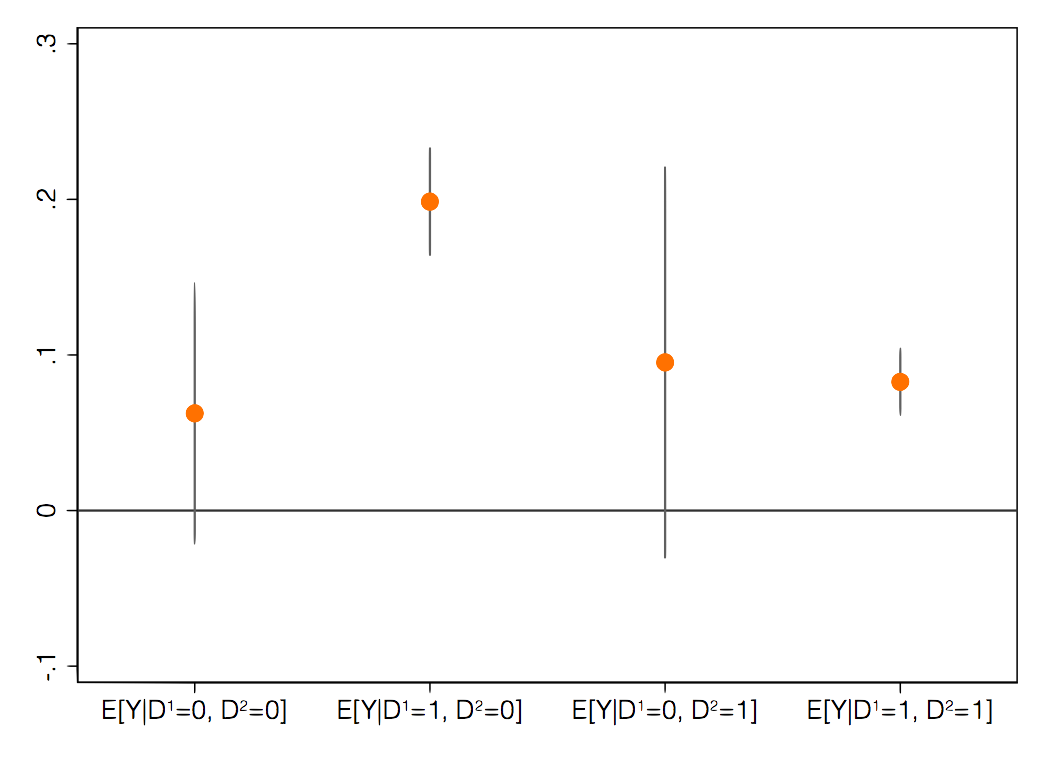
\includegraphics[height=.7\textheight,keepaspectratio=true]{../04-figures/10/05-w10_treatreat}
    \end{figure}
    
\end{frame}




\begin{frame}
  \frametitle{Calculating and plotting CATEs}
\footnotesize

In treatment-by-treatment interactions, we will usually also be interested in pairwise comparisons and their significance, i.e.\ the question whether the estimated effects just shown are significantly different \textcolor{orange}{from each other}:
\vspace{5mm}

\tiny
\centering
\begin{tabular}{ll}
Pairwise comparison & Associated hypothesis test \\
\midrule
$(E[Y_i|D_i^1=0, D_i^2=0]$ vs.\ $(E[Y_i|D_i^1=1, D_i^2=0]$ & $H0: \beta_0 - (\beta_0 + \beta_1) = 0$ \\
$(E[Y_i|D_i^1=0, D_i^2=0]$ vs.\ $(E[Y_i|D_i^1=0, D_i^2=1]$ & $H0: \beta_0 - (\beta_0 + \beta_2) = 0$ \\
$(E[Y_i|D_i^1=0, D_i^2=0]$ vs.\ $(E[Y_i|D_i^1=1, D_i^2=1]$ & $H0: \beta_0 - (\beta_0 + \beta_1 + \beta_2 + \beta_3) = 0$ \\
$(E[Y_i|D_i^1=1, D_i^2=0]$ vs.\ $(E[Y_i|D_i^1=0, D_i^2=1]$ & $H0: \beta_0 + \beta_1 - (\beta_0 + \beta_2) = 0$ \\
$(E[Y_i|D_i^1=1, D_i^2=0]$ vs.\ $(E[Y_i|D_i^1=1, D_i^2=1]$ & $H0: \beta_0 + \beta_1 - (\beta_0 + \beta_1 + \beta_2 + \beta_3) = 0$ \\
$(E[Y_i|D_i^1=0, D_i^2=1]$ vs.\ $(E[Y_i|D_i^1=1, D_i^2=1]$ & $H0: \beta_0 + \beta_2 - (\beta_0 + \beta_1 + \beta_2 + \beta_3) = 0$
\end{tabular}

\flushleft\footnotesize
Note: Once we do these multiple comparisons, we have to start worrying about `fishing' for statistically significant differences (more below)
\vspace{1cm}

\end{frame}




\begin{frame}
  \frametitle{Calculating and plotting CATEs}
\footnotesize

What if the modifying variable is \textcolor{orange}{continous}?

For example, consider the model: 

$Y_i = \beta_0 + \beta_1 {BB} + \beta_2 {Age}_i + \beta_3 {Age}_i \times {BB}_i + \epsilon_i$

where ${BB}$ indicates broadband availability, which can be high (1) or low (0), and ${Age}$ is a continuous variable recording an individual's age.

\vspace{3cm}

\end{frame}



\begin{frame}
  \frametitle{Calculating and plotting CATEs}
\footnotesize
The corresponding regression table looks as follows:

\tiny
\centering
\begin{tabular}{l*{1}{c}}
\toprule
\multicolumn{2}{c}{Conditional effect of broadband access on right-wing support}\\
\midrule
BB ($\beta_1$)             &    0.327\textsuperscript{***}\\
                &   (0.09)         \\
Age ($\beta_2$) &    0.002         \\
                &   (0.00)         \\
BB $\times$ Age ($\beta_3$) &   -0.005\textsuperscript{**} \\
                &   (0.00)         \\
Constant ($\beta_0$)  &   -0.039         \\
                &   (0.08)         \\
\midrule
Observations    &     1,158         \\
\(R^{2}\)       &     0.03         \\
\bottomrule
\multicolumn{2}{l}{Standard errors in parentheses}\\
\multicolumn{2}{l}{\textsuperscript{*} \(p<0.10\), \textsuperscript{**} \(p<0.05\), \textsuperscript{***} \(p<0.01\)}\\
\end{tabular}

\flushleft\footnotesize
Note that here the constitutive term $\beta_1$ indicates the effect of broadband access when age is zero -- it basically has no substantively interesting interpretation: calculation of marginal effects is mandatory in this case. 

\footnotesize


\end{frame}



\begin{frame}
  \frametitle{Calculating and plotting CATEs}
\footnotesize

The table below shows marginal effects for individuals aged 20, 30, 40, 50, 60, and 70.

\tiny
\centering
\begin{tabular}{l*{1}{c}}
\toprule
\multicolumn{2}{c}{Marginal effects of broadband access on right-wing support}\\
\midrule
Age = 20          &    0.221\textsuperscript{***}\\
                &   (0.05)         \\
Age = 30          &    0.169\textsuperscript{***}\\
                &   (0.04)         \\
Age = 40          &    0.116\textsuperscript{***}\\
                &   (0.03)         \\
Age = 50          &    0.064         \\
                &   (0.04)         \\
Age = 60           &    0.011         \\
                &   (0.06)         \\
Age = 70          &   -0.041         \\
                &   (0.07)         \\
\midrule
Observations    &     1,158         \\
\bottomrule
\multicolumn{2}{l}{Standard errors in parentheses}\\
\multicolumn{2}{l}{\textsuperscript{*} \(p<0.10\), \textsuperscript{**} \(p<0.05\), \textsuperscript{***} \(p<0.01\)}\\
\end{tabular}

\end{frame}



\begin{frame}
  \frametitle{Calculating and plotting CATEs}
\footnotesize

For effective communication, the best practice is to plot the results:

	 \begin{figure} 
    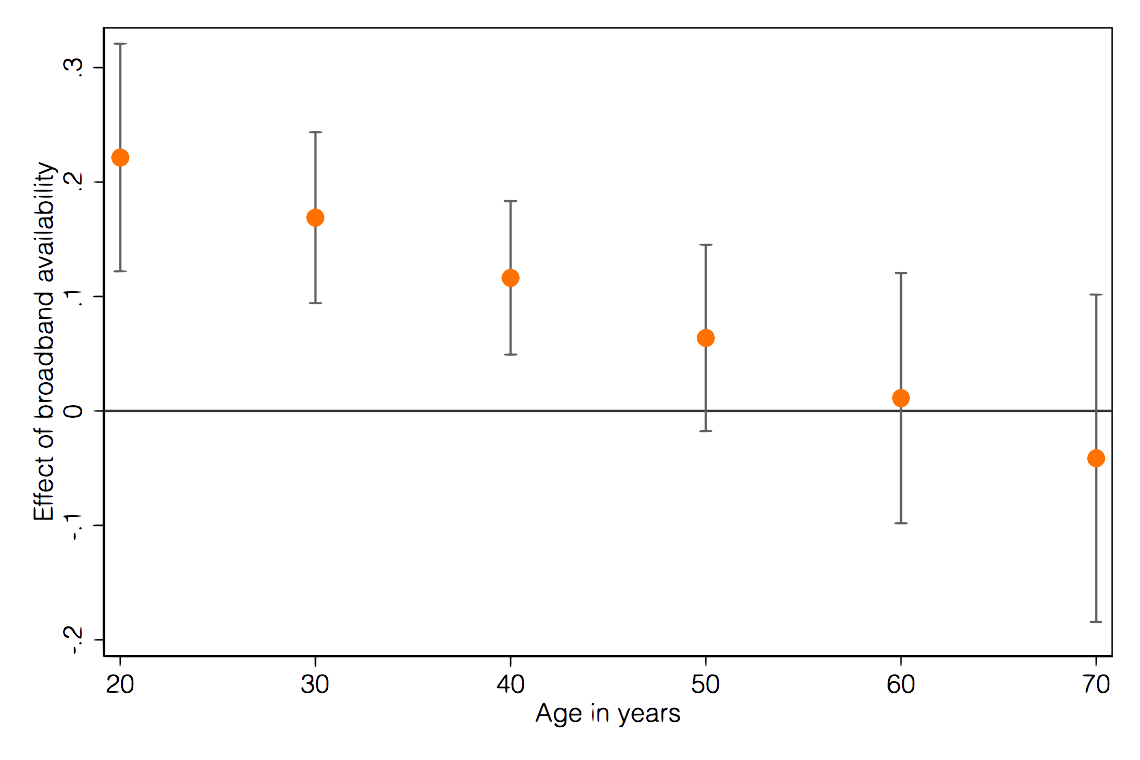
\includegraphics[height=.65\textheight,keepaspectratio=true]{../04-figures/10/06-w10_continuous}
    \end{figure}
    
\end{frame}



\begin{frame}
  \frametitle{Some caveats with regard to moderation analysis}
\footnotesize

Heterogeneous treatment effects can convey very important information that is often highly policy relevant. 

However, they are often seen with skepticism by the research community.

This is because of the problem of `fishing': with the number of heterogeneous treatment effects calculated, the likelihood of finding a significant effect grows.

Assuming the conventional p-value of 0.05 used to mark findings as `significant', 1/20 coefficients will be statistically significant \emph{by chance alone}. 

This opens the possibility for researchers to calculate many heterogeneous effects, and to seek out and report `significant' ones \cite{humphreys_fishing_2013}.

\end{frame}


\begin{frame}
  \frametitle{Some caveats with regard to moderation analysis}
\footnotesize
Several solutions to the `multiple-comparison' problem have been proposed: 

\begin{enumerate}
\item[1.] Statistical control, e.g.\ Bonferroni correction: for each comparison you do, the critical value against which a result is found to be significant is reduced. 

For example, if 4 values are reported, coefficients should meet the critical p-value of 0.05/4=0.0125 to be considered statistically significant. While rigorous, this test is often considered too conservative.
\end{enumerate}

\vspace{1cm}
\end{frame}


\begin{frame}
  \frametitle{Some caveats with regard to moderation analysis}
\footnotesize

\begin{enumerate}
\item[2.] Automate the search for treatment effects using vector machines (R::FindIt), Bayesian additive regression trees (R::BayesTree), classification and regression trees (R::causalTree), random forests, and kernel regularized least squares (R::KRLS);

These methods can 1) help to find the most important splits in the data, and 2) take discretion away from the researcher, thereby alleviating concerns with `fishing' -- however, they are atheoretical and may `miss' finding heterogeneity -- or the absence of it! -- in groups that are important for policy makers.
\end{enumerate}

\vspace{2cm}
\end{frame}

\begin{frame}
  \frametitle{Some caveats with regard to moderation analysis}
\footnotesize

\begin{enumerate}
\item[3.] Preregistration: researchers pre-register the comparisons and splits of the data they intend to investigate \emph{before} collecting and/or analyzing the data; i.e.\ they `bind their hands' as to which results they will present. 

This idea has become very popular. Also, writing a preregistration plan is very good practice for laying out your hypotheses \emph{before} you start collecting data.
\end{enumerate}

\vspace{2cm}
\end{frame}


\begin{frame}
  \frametitle{Some caveats with regard to moderation analysis}
\footnotesize

Moderation analysis is often used as a way to test for \textcolor{orange}{causal mechanisms}. 

The idea is that if the treatment effect varies strongly along an interacted variable, that variable must have \emph{something} to do with the underlying causal mechanism.

As stated, this type of logic is at best highly informal, and at worst throughly misleading. 

The only case where moderation can be used in the analysis of mechanisms in a rigorous fashion is when the stipulated mechanism is turned into a treatment, and treatment-by-treatment interactions are calculated.

Otherwise, the formal analysis of causal mechanisms is the domain of mediation analysis. 

\vspace{1cm}
\end{frame}




% END
\begin{frame}
\begin{center}
    \LARGE Thank you for watching, and see you next Monday!
\end{center}
\end{frame}

% REFERENCES %

\begin{frame}[allowframebreaks]
\frametitle{References}
\bibliographystyle{apacite}
\scriptsize\bibliography{../Bibliography}
\end{frame}

\end{document}
